\documentclass{article}
\usepackage[margin=3cm]{geometry}
\usepackage{amssymb}

% Figures
\usepackage{graphicx}
\usepackage{color}

% Page formatting
\newsavebox{\notetitle}
\newsavebox{\noteauthor}
\newsavebox{\notenumber}
\newsavebox{\notedate}
\renewcommand{\title}[1]{\sbox{\notetitle}{\Large{\textbf{#1}}}}
\renewcommand{\author}[1]{\renewcommand{\and}{\quad}\sbox{\noteauthor}{\large{#1}}}
\renewcommand{\date}[1]{\sbox{\notedate}{\large{#1}}}
\newcommand{\nb}[1]{\sbox{\notenumber}{\Large{\textbf{#1}}}}
\newcommand{\makemadtitle}{
  \hrule
  \vspace{.5em}
  \noindent
  \begin{center}
  \textbf{
  {\centering
\includegraphics[height=3cm]{../logoCHISTERA2014}}\\
   {\centering\Large COACHES project, CHIST-ERA 2014 program}
  }
  \end{center}
  \vspace{.5em}
 
  \hrule
  \vspace{3em}
  \begin{center}
    \begin{large}\textbf{ Note~\usebox{\notenumber}.}\end{large}\\[.5em]
    \begin{Large}\textbf{\usebox{\notetitle}}\end{Large}\\[2em]
    \begin{large}\usebox{\noteauthor} --- \usebox{\notedate}\end{large}
  \end{center}
  \vspace{3em}
}

% Various macros and environments
\newtheorem{prop}{Proposition}
\newtheorem{proposition}[prop]{Proposition}
\newtheorem{defn}{Definition}
\newtheorem{definition}[defn]{Definition}
\newtheorem{cor}{Corollary}
\newtheorem{corollary}[cor]{Corollary}
\newtheorem{exmp}{Example}
\newtheorem{example}[exmp]{Example}
\newtheorem{lem}{Lemma}
\newtheorem{lemma}[lem]{Lemma}
\newtheorem{fact}{Fact}
\newtheorem{thm}{Theorem}
\newtheorem{theorem}[thm]{Theorem}
\newtheorem{prob}{Problem}
\newtheorem{problem}[prob]{Problem}
\newtheorem{rem}{Remark}
\newtheorem{remark}[rem]{Remark}
\newtheorem{conj}{Conjecture}
\newtheorem{conjecture}[conj]{Conjecture}
\newenvironment{pf}{{\bf Proof }}{\hfill$\Box$\par}
\newenvironment{proof}{{\bf Proof }}{\hfill$\Box$\par}
\newcommand{\spaceafterproof}{\vspace{1em}}

% NOTE ITSELF BELOW %%%%%%%%%%%%%%%%%%%%%%%%%%%%%%%%%%%%%%%%%%%%%

\title{ Defintions of tasks and dialogues}
\author{COACHES Consortium: Abdel-Illah Mouaddib, Luca Iocchi, Laurent Jeanpierre}
\nb{: Technical report WP4 and WP3}

\date{\today}

\begin{document}

\includegraphics[height=2cm]{../logoUNICAEN.jpg}

\includegraphics[height=2cm]{../logoSapienza.png}
\includegraphics[height=2cm]{logo-vub}

\includegraphics[height=2cm]{logoSebanci}


\makemadtitle

\vspace*{1.0in}
\begin{abstract}
 This document describes the fundamental elements for the decision making module and its interaction with the interaction module. 
  \end{abstract}

\vspace*{1.5in}

\fbox{
\begin{minipage}{1.0\textwidth}
\begin{center}
 $\copyright$, THE COACHES CONSORTIUM \\
The copyright in this document is the property of the COACHES Consortium. This document is supplied by the COACHES consortium on the express terms that it is to be treated as confidential. This document is not external distribution without the project manager's permission. 
\end{center}
\end{minipage}
}
\newpage
\section{Introduction}
This document consists of describing different tasks that we will consider in the project and dialogues between the robots and the human (visitors, shopkeepers and the security unit).  The general framework consists of a communication between the knowledge-based module (WP1) and the decision module (WP4) where the decision module receives a set of goals to accomplish based on the reasoning of the KB module using different information, features and requests coming from sensors and the interaction module (WP3). The decision module develop a policy to select the goal to accomplish and how to accomplish it. This policy dictates to the robots to act by navigating, advertising (or both at the same time), to initiate a dialogue, or to patrol. All the these tasks will be described in the following. 
\section {Basic principles}
Robots receive from KB module a set of goals $G = \{ g_{1}, g_{2}, \ldots, g_{k} \}$ where goals concern advertisement, patrolling, assisting and escorting.  We note also that advertising goals could be performed in parallel with the moving goal. That�s why, we consider an incremental structure of tasks IST, inspired from progressive processing units. Indeed, we define four IST or each kind of goals. Each IST is composed of levels where the first level concern goto site $X$, the second level concern do advertisement at a location $(x,y)$ and do $X$ which concerns the assistance, the patrolling or the escorting. In addition to that, we consider some joint goals requiring joint IST.  For example, escorting a people from one location in a building to another location in the other building, this requires a cooperation between robots. Indeed, the first robot execute a policy of IST escorting the people to the exit of the first building, provide him information to reach the other building and then send information to the other robots in the other building to continue the escorting task at the second building. The structure of tasks we propose is as follows \{goto $x$, advertisement, do $x$ \} and for the joint task {\sc \{ goto $x$, advertisement, inform people, send message to the other robots \}} . Do $x$ concerns different tasks of assistance. That we develop in the following. 

%\begin{figure}[htbp]
%\begin{center}
%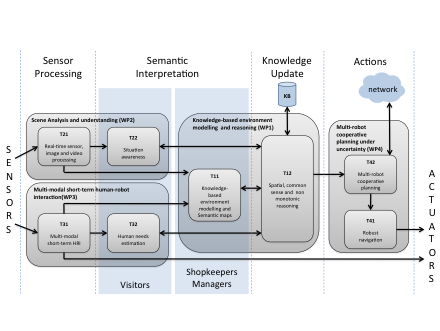
\includegraphics[height=10cm]{ArchitectureCoachesDF}
%\caption{Architecture and data flow }
%\label{Fig-1}
%\end{center}
%\end{figure}
\section {Description of Tasks}

The global structure of tasks will be based on a hierarchy of modules to execute: 

\begin{figure}[htbp]
\begin{center}
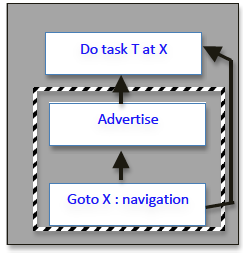
\includegraphics[height=10cm]{GeneralTask}
\caption{General task structure }
\label{FigTaskstructure}
\end{center}
\end{figure}

The two subtasks goto and advertise are supposed to be executed in parallel where goto $X$ is a subtask sent to the module navigation for execution and advertise is sent to the module multi-modale interaction for advertisement considering the current location of the robot. This subtask is optional and the human can stop the advertisement when needed. 

This structure will serve to express different tasks that we consider in the project: 
\begin{enumerate}
\item {\it Assistance Task (AT)}: this task consists in joining the location of the person and then use a dialogue subtask to exchange with him to make clear his needs. The structure of the task. Dialogue can concern: showing a direction, searching a shop, advertise and transporting goods. The schema of this dialogue is given in the next section.
\begin{figure}[htbp]
\begin{center}
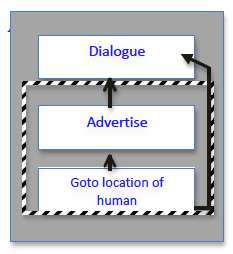
\includegraphics[height=10cm]{AssistanceTask}
\caption{Assistance task }
\label{FigAssistanceTask}
\end{center}
\end{figure}
\item {\it Escorting task (ET)}: this task consists of joining the person and escorting him to his target destination by maintaining the joint intention. When the behavior of the human is not appropriate, a dialogue between the robot and him js performed. This dialogue is described in the next section. 
\begin{figure}[htbp]
\begin{center}
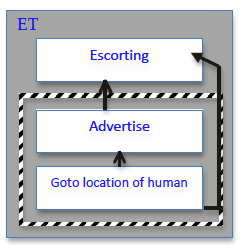
\includegraphics[height=10cm]{EscortingTask}
\caption{Escort task }
\label{FigEscortTask}
\end{center}
\end{figure}

\item {\it Collaborative Task (CT)}: this task consists in joining the location execute the part of the task, send message to the other robots during the travel and then inform the person.
\begin{figure}[htbp]
\begin{center}
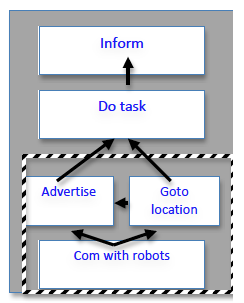
\includegraphics[height=10cm]{JointTask}
\caption{Joint task }
\label{FigjointTask}
\end{center}
\end{figure}
\item {\it Welcoming visitor task  (PT)}: this task consists in going to the entrance and initiating a dialogue with a visitor. The dialogue is described bellow  and is the same as for assistance task. 
\begin{figure}[htbp]
\begin{center}
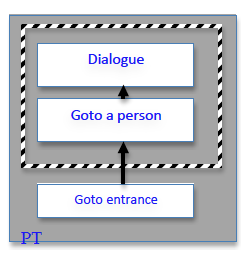
\includegraphics[height=10cm]{patrolTask}
\caption{Patrol task }
\label{FigPatrolTask}
\end{center}
\end{figure}
\item {\it Surveillance task (ST)}: this task consists in heading a destination where an abnormal object has been detected, taking a picture, send it and then call the security unit when informing people to be away from this object. 
\begin{figure}[htbp]
\begin{center}
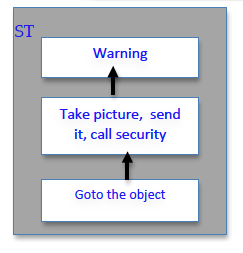
\includegraphics[height=10cm]{SecurityTask}
\caption{Security  task }
\label{FigsecurityTask}
\end{center}
\end{figure}
\end{enumerate}

\section{Description of dialogue}
\subsection{Dialogue with visitor}
\begin{figure}[htbp]
\begin{center}
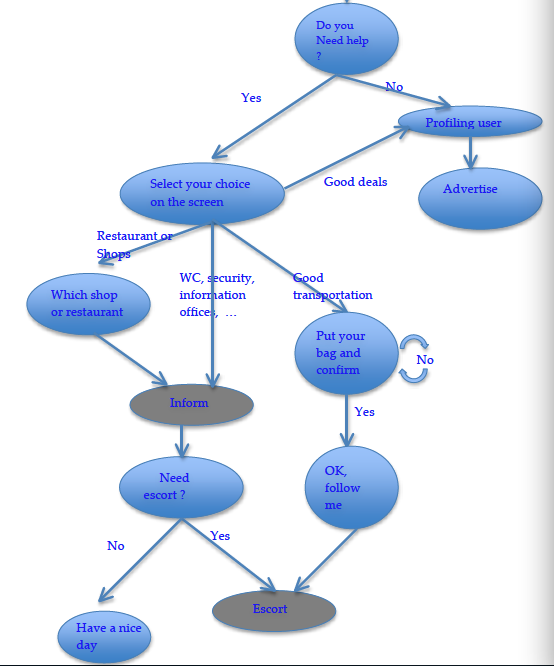
\includegraphics[height=20cm]{VisitorDialogueII}
\caption{Dialogue with visitor}
\label{FigVisitorDialogue}
\end{center}
\end{figure}
\subsection{Dialogue during escort}
\begin{figure}[htbp]
\begin{center}
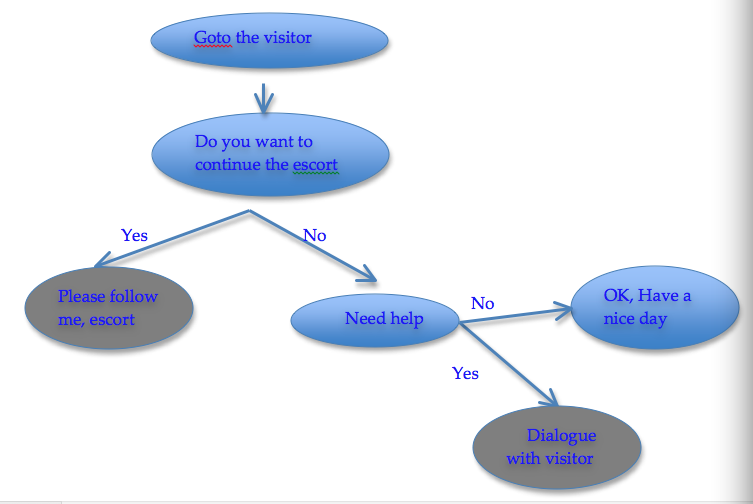
\includegraphics[height=12cm]{EscortDialogue}
\caption{Dialogue with visitor during the escort}
\label{FigVisitorDialogueII}
\end{center}
\end{figure}
\subsection{Dialogue with shopkeepers}
\begin{figure}[htbp]
\begin{center}
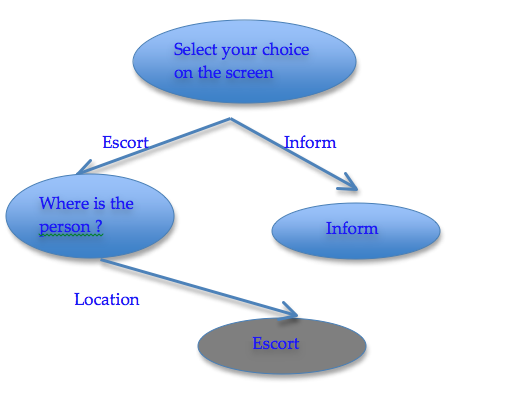
\includegraphics[height=15cm]{VisitorDialogue}
\caption{Dialogue with Shopkeepers}
\label{FigVisitorDialogue}
\end{center}
\end{figure}

\end{document}
